\section{\normalsize Зависимость давления насыщенного пара от кривизны поверхности жидкости. Кипение. Роль	зародышей в образовании новой фазы. }
\paragraph{Зависимость давления насыщенного пара от кривизны поверхности жидкости.} Пусть капля находится в состоянии равновесия и имеет форму шара, радиуса $r$.\\
По формуле Лапласа $P_\text{ж.}-P_\text{п.}=\dfrac{2\sigma}{r}.$ В состоянии термодинамического равновесия химические потенциалы $\left(\frac{\Phi}{N}\right)$ равны: $\varphi_\text{ж.}(P_\text{ж.},T)=\varphi_\text{п.}(P_\text{п.},T)$. \\В случае плоской поверхности раздела, когда давление насыщенного пара $P_0$:\\ $\varphi_\text{ж.}(P_0,T)=\varphi_\text{п}(P_0,T)\Rightarrow\varphi_\text{ж.}(P_\text{ж.},T)-\varphi_\text{ж.}(P_0,T)=\varphi_\text{п.}(P_\text{п.},T-\varphi_\text{п}(P_0,T)).$\\ 
Считая $P_\text{ж.}-P_0$ и $P_\text{п.}-P_0$ малыми: $(P_\text{ж.}-P_0)\chpr{\varphi_\text{ж.}}{P}{T}=(P_\text{п.}-P_0)\chpr{\varphi_\text{п.}}{P}{T}$\\
$d\varphi=-sdT+vdP\Rightarrow\chpr{\varphi}{P}{T}=v\Rightarrow(P_\text{ж.}-P_0)v_\text{ж.}=(P_\text{п.}-P_0)v_\text{п.}\Rightarrow$
\begin{equation*}
\Rightarrow
\begin{cases}
P_\text{ж.}-P_0=\dfrac{v_\text{п.}}{v_\text{п.}-v_\text{ж.}}\dfrac{2\sigma}{r}\simeq\dfrac{2\sigma}{r}\longrightarrow P_\text{ж.}=P_0+\dfrac{2\sigma}{r}\\
P_\text{п.}-P_0=\dfrac{v_\text{ж.}}{v_\text{п.}-v_\text{ж.}}\dfrac{2\sigma}{r}\simeq\dfrac{v_\text{ж.}}{v_\text{п.}}\dfrac{2\sigma}{r}\longrightarrow P_\text{п.}=P_0+\dfrac{v_\text{ж.}}{v_\text{п.}}\dfrac{2\sigma}{r}
\end{cases}
\end{equation*}
$P_\text{п.}=P_0+\dfrac{v_\text{ж.}}{v_\text{п.}}\dfrac{2\sigma}{r}\text{ --- давление пара над искривленной поверхностью капли в воздухе}$. Формальной заменой $r$ на $(-r)$ получаем:
$$P_\text{ж.}=P_0-\dfrac{2\sigma}{r}$$
$$P_\text{п.}=P_0-\dfrac{v_\text{ж.}}{v_\text{п.}}\dfrac{2\sigma}{r}=P_0-\dfrac{\rho_\text{п.}}{\rho_\text{ж.}}\dfrac{2\sigma}{r}$$
$$P_\text{п.}=P_0-\dfrac{\rho_\text{п.}}{\rho_\text{ж.}}\dfrac{2\sigma}{r}\text{ --- давление пара под искривленной поверхностью пузырька в жидкости.}$$
Но $P_\text{п.}-P_0$ не всегда мала, тогда считая пар идеальным газом можем получить следующую выкладку: $v=\dfrac{RT}{P};\ d\varphi=-sdT+vdP$, при $T=const$: $\varphi_\text{п.}(P_\text{п.},T)-\varphi_\text{п.}(P_0,T)=RT\ln\left(\dfrac{P_\text{п.}}{P_0}\right)$\\
$v_\text{ж.}(P_\text{ж.}-P_0)=RT\ln\left(\dfrac{P}{P_0}\right)\Leftrightarrow v_\text{ж.}\left(P_\text{п.}-P_0-\dfrac{2\sigma}{r}\right)=RT\ln\left(\dfrac{P}{P_0}\right)$ и при $P_\text{п.}-P_0\ll\dfrac{2\sigma}{r}:$
$$P_\text{п.}=P_0\exp\left[-\dfrac{2\sigma v_\text{ж.}}{RTr}\right]\Leftrightarrow \underline{P_\text{п.}=P_0\exp\left[-\dfrac{2\sigma}{P_0r}\dfrac{v_\text{ж.}}{v_\text{п.}}\right]}$$
\paragraph{Кипение.} Фазовые переход, происходящий с образованием пузырьков пара по всему объему жидкости называется \textbf{кипением}, относится к фазовым переходам первого рода. Температура, при которой кипит жидкость при \underline{$P=const$} --- \textbf{температура кипения}. Кипение может начинаться при тех температурах, когда вместе могут существовать жидкая и парообразная фазы, т.е. $P_\text{н.п.}=P_\text{внеш.}=P_0$ при этом $P(T)=P_0\exp\left[\dfrac{q_\text{м.}}{RT_0}-\dfrac{q_\text{м.}}{RT}\right]$,\\
где $q_\text{м.}$ --- молярная теплота парообразования. Тогда
$$T=\dfrac{T_0}{1-\frac{RT_0}{q_\text{м.}}\ln\left(\frac{P}{P_0}\right)}\text{ --- зависимость $T_\text{кип.}$ от $P$}$$ 
Найдем \textbf{критический размер пузырька пара в жидкости}. Пусть однородная жидкость находится в метастабильном состоянии. Будем наблюдать за пузырьком пара в ней.\\
$P_\text{ж.}=P_\text{атм.}+P_\text{гидростат.}=const$, значит однозначно задается $P_\text{п. и }r$
\begin{equation*}
\begin{cases}
P_\text{п.}=P_\text{ж.}+\dfrac{2\sigma}{r}\\
P_\text{п.}=P_0(T)-\dfrac{v_\text{ж.}}{v_\text{п.}-v_\text{ж.}}\dfrac{2\sigma}{r}
\end{cases}
\longrightarrow r_\text{кр.}=\dfrac{2\sigma}{P_0(T)-P_\text{ж.}}\dfrac{v_\text{ж.}}{v_\text{п.}-v_\text{ж.}}
\end{equation*}

\begin{wrapfigure}{L}{42mm}
	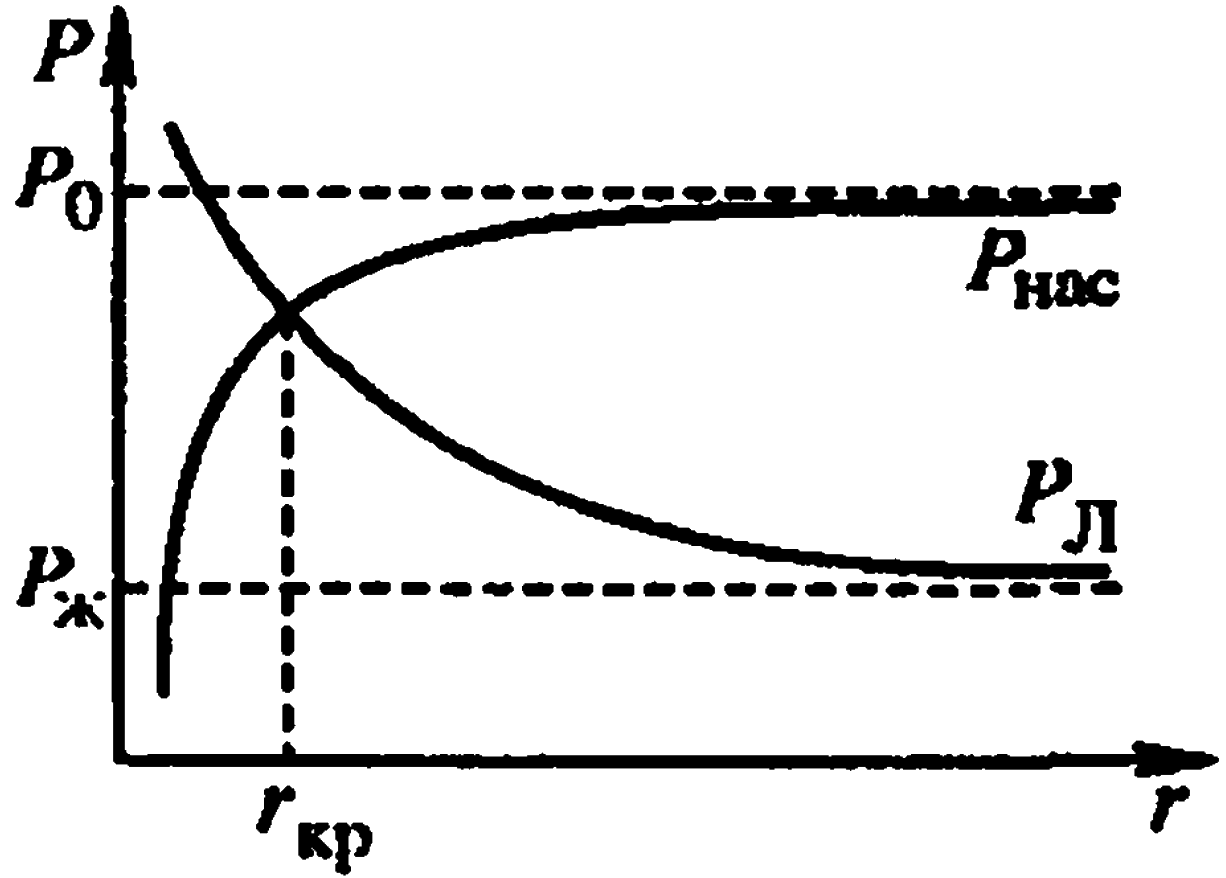
\includegraphics[width=42mm]{ris24.png}
\end{wrapfigure}
$$r_\text{кр.}\simeq\dfrac{2\sigma}{P_0(T)-P_\text{ж.}}\textbf{ --- критический размер пузырька}$$
При $r<r_\text{кр. }P_\text{нас.}<P_\text{лап.}\rightarrow$ пузырек не выдерживает и схлопывается.\\
При $r>r_\text{кр. }P_\text{нас.}>P_\text{лап.}\rightarrow$ пузырек начинает расти.\\[0.5cm]
Аналогичный случай --- капля воды в переохлажденном паре
$$r_\text{кр.}\simeq\dfrac{2\sigma}{P_0(T)-P_\text{п.}}\dfrac{v_\text{ж.}}{v_\text{п.}}$$
$r<r_\text{кр.}$ --- капля испарится, $r\geqslant r_\text{кр}$ --- будет расти.
\paragraph{Роль	зародышей в образовании новой фазы.} Если в очищенную от посторонних примесей воду, которая остается жидкой при $t=-10^\circ C$ и ниже бросить кристаллик льда (\textbf{зародыш} кристаллической фазы) или встряхнуть сосуд, то вода быстро затвердеет и ее температура быстро поднимется до $0^\circ C$. Если же она не была очищена от посторонних вкраплений, способных выполнять функцию зародыша кристаллической фазы, то переохлаждение наблюдаться не будет. (Подробнее --- Сивухин стр. 465-466).
